\documentclass[a4paper,12pt]{book} %文档类型
\usepackage{xeCJK}
\usepackage{ctex}
\usepackage{amsmath,amssymb,amstext} %多种公式环境和数学命令
\usepackage{amsthm}
\usepackage{float}
\usepackage[font=small,labelsep=quad]{caption}
\usepackage{epstopdf}
\usepackage{array}           %数组和表格制作
\usepackage{fancyhdr}        %页眉页脚设置
\usepackage{graphicx}        %插图
\usepackage{subfigure}
\usepackage{tabularx}        %自动设置表格列宽
\usepackage{multirow}        %跨行表格
\usepackage{multicol}        %跨列表格
\usepackage{titlesec}        %标题设置
\usepackage{titletoc}        %目录格式设置
\usepackage{url}
\usepackage{listings}
\usepackage{clrscode3e}
\lstset{breaklines}%自动将长的代码行换行排版
\lstset{extendedchars=false}%解决代码跨页时,章节标题,页眉等汉字不显示的问题
\usepackage{booktabs}
\usepackage[top=2.5cm,bottom=2.5cm,left=2.0cm,right=2.0cm]{geometry} % 页边距
\renewcommand{\figurename}{{图}}
\renewcommand{\tablename}{{表}}
\linespread{1.4}   %1倍行距
\usepackage{xcolor}
\usepackage{courier}
\usepackage{hyperref}
\lstset{
    numbers=left, %设置行号位置
    numberstyle=\small\ttfamily, %设置行号大小
    basicstyle=\small\ttfamily, %设置一般字颜色
    keywordstyle=\small\ttfamily\color{blue}, %设置关键字颜色
    identifierstyle=\small\ttfamily, %设置标识符颜色
    stringstyle=\small\ttfamily, %设置字符串颜色
    commentstyle=\color[cmyk]{1,0,1,0}, %设置注释颜色
    breaklines, %自动折行
    extendedchars=false, %解决代码跨页时,章节标题,页眉等汉字不显示的问题
    showstringspaces=false, %不显示代码字符串中间的空格标记
    tabsize=4,
}
\usepackage{verbatim}
\usepackage{setspace}
\usepackage{algorithm}
\usepackage{algpseudocode}
\usepackage{algorithmicx}
\renewcommand{\algorithmicrequire}{\textbf{Input:}}  % Use Input in the format of Algorithm  
\renewcommand{\algorithmicensure}{\textbf{Output:}} % Use Output in the format of Algorithm  
\usepackage{bbm}
\usepackage{times}
\usepackage{fontspec}
\setmainfont{Times New Roman}
\usepackage{tikz}
\usetikzlibrary{arrows, automata}
\newcommand\myVSpace[1][0pt]{\rule[\normalbaselineskip]{0pt}{#1}}

\setCJKfamilyfont{zhsong}{STSong}
\setCJKfamilyfont{zhhei}{STHeiti}
\setCJKfamilyfont{zhkai}{STKaiti}

\newcommand*{\song}{\CJKfamily{zhsong}} % 宋体
\newcommand*{\hei}{\CJKfamily{zhhei}}   % 黑体
\newcommand*{\kai}{\CJKfamily{zhkai}}  % 楷书

\newcommand{\yihao}{\fontsize{26pt}{36pt}\selectfont}           % 一号, 1.4 倍行距
\newcommand{\erhao}{\fontsize{22pt}{28pt}\selectfont}          % 二号, 1.25倍行距
\newcommand{\xiaoer}{\fontsize{18pt}{18pt}\selectfont}          % 小二, 单倍行距
\newcommand{\sanhao}{\fontsize{16pt}{24pt}\selectfont}        % 三号, 1.5倍行距
\newcommand{\xiaosan}{\fontsize{15pt}{22pt}\selectfont}        % 小三, 1.5倍行距
\newcommand{\sihao}{\fontsize{14pt}{21pt}\selectfont}            % 四号, 1.5 倍行距
\newcommand{\banxiaosi}{\fontsize{13pt}{19.5pt}\selectfont}    % 半小四, 1.5倍行距
\newcommand{\xiaosi}{\fontsize{12pt}{18pt}\selectfont}            % 小四, 1.5倍行距
\newcommand{\dawuhao}{\fontsize{11pt}{11pt}\selectfont}       % 大五号, 单倍行距
\newcommand{\wuhao}{\fontsize{10.5pt}{15.75pt}\selectfont}    % 五号, 单倍行距

\usepackage{CJKnumb}
\titleformat{\chapter}{\centering\zihao{3}\bfseries}{第\CJKnumber{\thechapter}章}{1em}{}
\titleformat*{\section}{\bfseries\zihao{4}}
\titleformat*{\subsection}{\bfseries\zihao{-4}}

\titlecontents{chapter}[0pt]
{\addvspace{2pt}\filright \bfseries \zihao{4}}
{\contentspush{\thecontentslabel ~~~}}{}{~\titlerule*[6pt]{.}\contentspage}
\titlecontents{section}[20pt]
{\bfseries \zihao{-4}}
{\contentspush{\thecontentslabel ~~~}}{}{~\titlerule*[6pt]{.}\contentspage}
\titlecontents{subsection}[16mm]
{\zihao{-4}}
{\contentspush{\thecontentslabel ~~~~}}{}{~\titlerule*[6pt]{.}\contentspage}

\usepackage{fancyhdr}
\pagestyle{fancy}
\renewcommand{\chaptermark}[1]{\markboth{第\CJKnumber{\thechapter}章~~~~#1}{}}
\fancyhead{}
\fancyhead[CO]{\zihao{-5} \leftmark}
%%%%%%%%%%%%%%%%%%%%%%%%%%%%%
%%%%% 请在下方键入论文标题 %%%%%
\fancyhead[CE]{\zihao{-5} 基于排队论的海韵二期小炒点餐策略研究}
%%%%% 请在上方键入论文标题 %%%%%
%%%%%%%%%%%%%%%%%%%%%%%%%%%%
\fancyfoot[CO]{\zihao{-5} \thepage}
\fancyfoot[CE]{\zihao{-5} \thepage}

\fancypagestyle{plain}{
    \lhead{} 
    \chead{} 
    \fancyfoot[CE,CO]{\zihao{-5} \thepage}
    \renewcommand{\headrulewidth}{0pt}
}

\begin{document}
\makeatletter
\newcommand\engcontentsname{Contents}
\newcommand\tableofengcontents{%
    \if@twocolumn
      \@restonecoltrue\onecolumn
    \else
      \@restonecolfalse
    \fi
    \chapter*{\engcontentsname
        \@mkboth{%
           \MakeUppercase\engcontentsname}{\MakeUppercase\engcontentsname}}%
    \@starttoc{toe}% !!!!Define a new contents!!!!
    \if@restonecol\twocolumn\fi
    }
\newcommand\addengcontents[2]{%
    \addcontentsline{toe}{#1}{\protect\numberline{\csname the#1\endcsname}#2}}
\makeatother

\newcommand\echapter[1]{\addengcontents{chapter}{#1}}
\newcommand\esection[1]{\addengcontents{section}{#1}}
\newcommand\esubsection[1]{\addengcontents{subsection}{#1}}

\captionsetup[table]{font={small, bf}}
\captionsetup[figure]{font={small, bf}}

\frontmatter
\pagenumbering{Roman}

%%%%%%%%%%%%%%%%%%%%%
%%%%% 以下为正文 %%%%%%
%%%%%%%%%%%%%%%%%%%%%

%----------------------------------------------
\chapter*{致谢}
\thispagestyle{plain}

又是一年凤凰花开,只是这一次是被海韵二期食堂的油烟熏开的。四年的时光总算过去了,回想起来,我已经享受了四载“家的味道”。什么是家?家是万能的芹菜,总能搭配各式各样的火锅料;家是平淡无味的盐,总能让方便面的本味不被遮盖;家是无人问津的炖罐,总能在你需要紫菜蛋汤时过来给你提供温馨的服务。没有这个家,四年光阴我是绝对无法肚过的。感谢这个充满油烟味的家,让我的生活始终接地气,让我没有在早上懒床后吃不了早饭饿着去上三四节课,让我在吃腻了外卖后还能找回点外卖的那份冲动。谢谢家里的每一名阿姨,是你们用颤抖的双手避免我们肥胖;谢谢家里的管家,总能适时扼住那双抖动的手让我在饥寒交迫中多一份热量;谢谢家里的大叔,让周润发式的叼烟在收盘处显得那么的迷人。

未来的路还很漫长,一路上还有很多的艰难险阻等着我们去面对。但是,我相信,“家人”早就通过种种方式告诉了我,该怎样面对:生活如紫菜海蛎煲,总是会有一粒粒恼人的沙子,虽小却让我们心生不快;生活如粉条兔肉,好解决的粉条永远是少,而难啃的兔肉却非常大;生活如免费汤,好东西永远需要我们悉心寻找才能发现。谢谢你们有这样生动的方式教会我这些人生哲理。

难说再见,外卖难点;难说再见,饭店太远;难说再见,菜永不变。我爱你,再见!\\

\rightline{\kai 小炒一霸~~~~于海韵}
\rightline{\kai 二〇一八年五月}

\clearpage{\pagestyle{empty}\cleardoublepage}    % 用于清除偶数空白页的页眉页脚


%----------------------------------------------
\chapter*{摘要}

俗话说:“学好数理化,走遍天下都不怕”。学习好排队论对于减少在海韵二期小炒等餐时间有着巨大的帮助。本文正是在多年摸爬滚打的经验下,运用形式化语言对问题建模,基于排队论思想创造性的提出了“合插论”方法,极大的节约了同学们的等待时间。

我们将点餐的的同学分成四组——荤菜组、素菜组、焖煲组和煮汤组,分别构建一个负指数分布进行描述,至于怎么描述我也说不清楚,反正输入过程就是泊松流。

实验结果表明,我们的方法就是很棒棒,实际情况同瞎做的仿真结果基本吻合,实际中同学的最大等待时间只有半个小时,比最新的方法还要快两分钟。
\newline

\textbf{关键词}:点餐策略;排队论;海韵二期食堂;小炒

\clearpage{\pagestyle{empty}\cleardoublepage}


%----------------------------------------------
\chapter*{Abstract}

You know, it's impossible for you to wirte this abstract in English directly, beacuse your English is so bad that even words can't be spelled correctly. I bet you will use \textbf{\Large Baidu} translation service or \textbf{\Large Google} translation service, with the help of Youdao dictionary. If I don't bold these two words, I guess you will pass this part.

As the saying goes: "Learning mathematics and physics and chemistry is not afraid to travel all over the world." Studying the queuing theory has a great help in reducing the time of dinner in Haiyun's second stage. This article is based on many years of experience, using formal language to model the problem. Based on the queuing theory, it puts forward the "combination-insertion theory" method, which greatly saves the waiting time of the students.

We divided the classmates who ordered food into four groups - the amaranth group, the vegetarian group, the wolfberry group, and the soup group. They constructed a negative exponential distribution to describe them. As for how to describe me, I couldn't say clearly. Anyway, the input process is Poisson flow.

The experimental results show that our method is awesome, and the actual situation is basically consistent with the results of the simulation done by the students. In practice, the maximum waiting time of the students is only a half hour, which is two minutes faster than the latest method.

This abstract is automatically generated by Google translation.
\newline

\textbf{Keywords}: Food ordering strategy; Queuing theory; Haiyun II canteen; Small fry

\clearpage{\pagestyle{empty}\cleardoublepage}


%----------------------------------------------
%%% 中文目录 %%%
\tableofcontents

\clearpage{\pagestyle{empty}\cleardoublepage}


%----------------------------------------------
%%% 英文目录 %%%
\tableofengcontents

\clearpage{\pagestyle{empty}\cleardoublepage}



%----------------------------------------------
%%% 大戏拉开帷幕 %%%
\mainmatter

%----------------------------------------------
\chapter{绪论}
\echapter{Introduction}

\section{课题研究背景及意义}
\esection{Background and Significance of the Study}

伟大领袖毛主席教导我们:“身体是革命的本钱”\cite{momo2003}。人是铁,饭是钢,不吃好怎么为社会主义建设做贡献。颇具人文关怀的厦门大学为同学们开辟了海韵二期小炒窗口,满足同学们的刁钻口味。可是,由于人实在太多,排队等餐时间太长,一来浪费同学们午睡时间,导致下午五六节课都在睡觉;二来也让厨子们总是要大声叫号,不利于保护嗓子。为了解决这一对矛盾。我们提出了这个课题。

\begin{figure}[htbp]
\centering
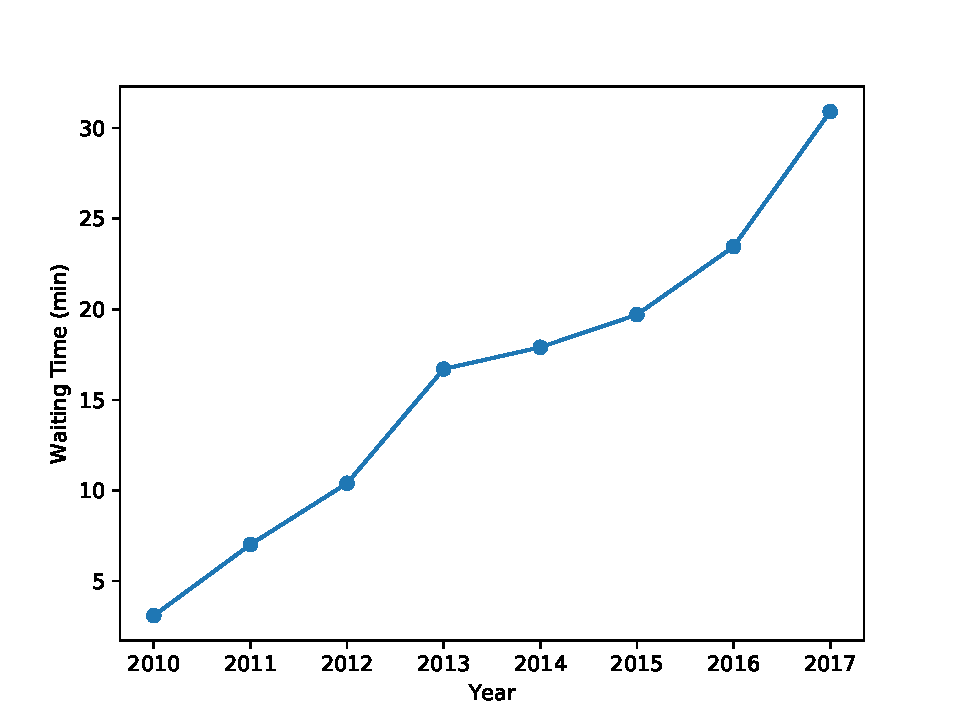
\includegraphics[width=0.8\textwidth]{sample_pic.pdf}
\caption{小炒的平均等待时间逐年增加}
\label{growth}
\end{figure}

我们初步统计了近几年的小炒窗口等待情况,计算了没一年的平均等待时间,得到了如图\ref{growth}所示的折线图。可以看出,随着时间的推移,同学们的平均等待时间越来越高,达到了惊人的半个小时!解决这个问题迫在眉睫。

\section{国内外研究现状}
\esection{Research Status at Home and Abroad}

国家膳食委员会与世界卫生组织在2017年7月曾对上海市和杭州市的各高校食堂特色窗口等待时间进行过统计\cite{Khan2006},结果发现绝大多数同学只需要1.3分钟就可以完成取餐。对比国内的情况,美国南加州大学和密歇根大学的研究人员对加州地区各大学的餐厅进行了调查研究,结果显示,有35\%的学生不能在半个小时内拿到食物 \cite{Marcus2015} 。还有哪些研究,我也不知道,谁这么无聊研究这种东西,如果有,那一定是读博士读得脑子抽风了,需要去仙岳医院看看医生。

下面就是凑数了,随便找几篇论文摘要抄抄,结论改改,就在这编,编够一百八十字,你就赢了。对了,记得抄英文论文,机器翻译一下,查重太傻,不会查出来的。

可是我要怎么才能凑够字数呢?我想想,我想想,我想想,我想想,我想想,我想想,我想想,我想想,我想想,我想想,我想想,我想想,我想想,我想想,我想想,我想想,我想想,我想想,我想想,我想想,我想想,我想想,我想想,我想想,我想想,我想想,我想想,我想想,我想想,我想想,我想想,我想想,我想想,我想想,我想想,我想想,我想想,我想想,我想想,我想想,我想想,我想想,我想想,我想想,我想想,我想想,我想想,我想想,我想想,我想想,我想想,我想想,我想想。不行,我不能再想了,脑仁要炸了。好吧,我决定了,抄抄文献!

食堂就餐排队模型探究很有必要性!

(1)从生活细节着手,构建和谐校园

食堂是学生就餐的场所,根据调查,在校学生选择 在食堂就餐的比例高达80\%以上,因此,如何确定最佳的窗口数量,让学生在最短时间内打到饭菜的同时又兼顾食堂的利益,是摆在眼前的一个非常现实的问题。学生食堂的存在和发展状况不仅关系到在校学生的生活问题,而且在某种程度上也关系到学生们的身体健康和学习状况。本研究通过构建一个简单的食堂排队模型,来解决学生就餐时排队等候时间过长的问题,从学生生活细节着手,为在校学生创造一个文明、和谐的就餐环境,有益于构建和谐校园。

(2)降低食堂管理成本,实现资源优化配置

食堂既是学校的硬件设施之一,又是学校管理的重要组成部分。通过对食堂排队模型的探究,得出食堂需要开设的窗口数量,有助于学校加强对食堂的管理,为进一步加强和改善食堂监管工作提供了依据。此外,通过排队模型得出最佳窗口数量,避免窗口开设过少致使学生排队等候时间过长以及开设窗口过多导致人力的浪费。因此,排队模型的建立与实现可以有效地降低食堂的管理成本,帮助实现资源的优化配置。

(3)响应国家政策,建设资源节约型社会

前国家主席胡锦涛在党的第十六届五中全会上强调要加快建设资源节约型社会,指出这是从我国国情出发的一项重大决策。食堂排队模型投入应用后,通过确定排队系统的各项特征,如平均等待时间、平均队长等,找出食堂应当开设的最佳窗口数量,防止人力、物力的双重浪费,有效地为资源的合理配置和有效利用提供科学依据。 

好吧,字数应该够了。可是这都是什么东西,高考思想政治都不能这么写啊,姐姐啊!

\section{研究内容及论文结构}
\esection{Main Contents and Structure of the Thesis}

你居然还不知道我要研究什么?你居然还不知道我要研究什么?你!居!然!还!不!知!道!我!要!研!究!什!么?难以置信!研究什么,我也说不清,你问我导师去吧,他让我研究的,我也没办法啊,不然我怎么毕业。

本文各章安排如下:

本章绪论,就是絮絮叨叨瞎扯淡。你就自己总结总结扯了啥吧。我是凑字数的,凑字数是我。我是凑字数的,凑字数是我。我是凑字数的,凑字数是我。我是凑字数的,凑字数是我。

第二章标题粘贴一下在这里,说了什么,我想想,我真的不清楚。好吧,我放弃了,我不干了,好烦。我是凑字数的,凑字数是我。我是凑字数的,凑字数是我。我是凑字数的,凑字数是我。我是凑字数的,凑字数是我。我是凑字数的,凑字数是我。我是凑字数的,凑字数是我。我是凑字数的,凑字数是我。我是凑字数的,凑字数是我。

第三章标题在此,你还想说些什么就说吧,反正没人看的。我是凑字数的,凑字数是我。我是凑字数的,凑字数是我。我是凑字数的,凑字数是我。我是凑字数的,凑字数是我。我是凑字数的,凑字数是我。我是凑字数的,凑字数是我。我是凑字数的,凑字数是我。我是凑字数的,凑字数是我。我是凑字数的,凑字数是我。我是凑字数的,凑字数是我。我是凑字数的,凑字数是我。

第四章实验结果与分析,就一个字,好!那必须是好啊,不好导师能放你走,答辩能放你走,学校能放你走?当然不可能,瞎编一个都要好。我是凑字数的,凑字数是我。我是凑字数的,凑字数是我。我是凑字数的,凑字数是我。我是凑字数的,凑字数是我。我是凑字数的,凑字数是我。

第五章总结与展望,总结了本文的主要研究工作,并对下一步工作进行了展望。展望你妹啊,劳资都要毕业了,还展望,延毕我啊!

\clearpage{\pagestyle{empty}\cleardoublepage}


%----------------------------------------------
\chapter{海韵二期小炒点餐策略研究的技术背景}
\echapter{Technical Background of Research of Food Order Strategy in Haiyun II Canteen}

\section{排队论}
\esection{Quene Theory}

排队论(Queuing theory), 或称随机服务系统理论, 是通过对服务对象到来及服务时间的统计研究,得出这些数量指标(等待时间、排队长度、忙期长短等)的统计规律,然后根据这些规律来改进服务系统的结构或重新组织被服务对象,使得服务系统既能满足服务对象的需要,又能使机构的费用最经济或某些指标最优。它是数学运筹学的分支学科。也是研究服务系统中排队现象随机规律的学科。广泛应用于计算机网络, 生产, 运输, 库存等各项资源共享的随机服务系统。 排队论研究的内容有3个方面:统计推断,根据资料建立模型;系统的性态,即和排队有关的数量指标的概率规律性;系统的优化问题。其目的是正确设计和有效运行各个服务系统,使之发挥最佳效益。

排队论起源于20世纪初的电话通话。1909—1920年丹麦数学家、电气工程师爱尔兰(A.K.Erlang)用概率论方法研究电话通话问题,从而开创了这门应用数学学科,并为这门学科建立许多基本原则。20世纪30年代中期,当费勒(W.Feller)引进了生灭过程时,排队论才被数学界承认为一门重要的学科。在第二次世界大战期间和第二次世界大战以后,排队论在运筹学这个新领域中变成了一个重要的内容。20世纪50年代初,堪道尔(D.G.Kendall)对排队论作了系统的研究,他用嵌入马尔柯夫(A.A.Markov)链方法研究排队论,使排队论得到了进一步的发展。是他首先(1951年)用3个字母组成的符号A/B/C表示排队系统。其中A表示顾客到达时间分布,B表示服务时间的分布,C表示服务机构中的服务台的个数。

排队系统由输入过程与到达规则、排队规则、服务机构的结构、服务时间与服务规划组成。一般还假设到达间隔时间序列与服务时间均为独立同分布随机变量序列,且这两个序列也相互独立。

评价一个排队系统的好坏要以顾客与服务机构两方面的利益为标准。就顾客来说总希望等待时间或逗留时间越短越好,从而希望服务台个数尽可能多些但是,就服务机构来说,增加服务台数,就意味着增加投资,增加多了会造成浪费,增加少了要引起顾客的抱怨甚至失去顾客,增加多少比较好呢?顾客与服务机构为了照顾自己的利益对排队系统中的3个指标:队长、等待时间、服务台的忙期(简称忙期)都很关心。因此这3个指标也就成了排队论的主要研究内容。

排队论的应用非常广泛,表\ref{table_ex}进行了总结。它适用于一切服务系统。尤其在通信系统、交通系统、计算机、存贮系统、生产管理系统等方面应用得最多。排队论的产生与发展来自实际的需要,实际的需要也必将影响它今后的发展方向。

\begin{table}[htbp]
\centering
\caption{我也不知道统计的是啥}
\label{table_ex}
\begin{tabular}{cccccc}
\toprule
\multirow{2}{*}{Heroes} & \multirow{2}{*}{Power} & \multicolumn{2}{c}{Life}   & \multicolumn{2}{c}{Speed} \\
                             &                          & Before & After & Before    & After    \\ \midrule
Dick                           & 34                     & 334            & 566              & 1.4                 & 4.8                  \\
Tommy                           & 76                      & 567             & 1888              & 1.1                 & 3.7                  \\
David                           & 22                     & 471            & 479             & 1.3                 & 3.4                  \\
Genia                           & 19                     & 1162          & 4273            & 1.7                & 6.7                \\
Hadoos                         & 55                        & 901               & 1589                 & 1.0                 & 3.0                  \\ \bottomrule
\end{tabular}
\end{table}

\section{还有啥技术背景}
\esection{No Background Here}

餐饮管理是指企业、医院、学校、酒店等根据需要将餐饮管理服务承包给专业的餐饮公司来管理,然后选择餐饮公司所提供的各类菜式就餐。

餐饮管理是一项集经营与管理、技术与艺术、秉承与创新于一体的业务工作,与其它部门的管理相比,具有不同的特点,要求饭店在餐饮管理上也应独具特色,以适应管理主体的要求。

制定出适合饭店自身的管理制度与方法,最重要的就是要认识各种管理制度和方法,了解各种制度产生的背景,深入研究各种制度适用的条件适合,不要先入为主。管理方法一定要适合饭店的环境,由于各饭店的环境不同,因此不可能有哪一种管理制度能适用于各饭店。即使在同一饭店内部,对不同部门的员工有时也要采用不同的管理方法。管理制度也有时间性,饭店住所的情况常随时间的不同而变化,管理制度和方法必须因时、因地、因人而变。

饭店一般采用的管理方法有:组织图表、工作种类、工作规范、工作时间表等等。

\subsection{组织图表}
\esubsection{Chart}
组织图表表示了岗位和职责的基本分类和关系,是组织形式的机构图,但有某些局限性,如各层次的职权范围和职责,地位相同的两个职员之间的非直线关系或不同部门的职员之间的间接关系皆不明显。由于这个原因,各种工作的描述和组织手册是对组织图标的重要补充说明。

\subsection{工作种类}
\esubsection{Type}
工作,种类是反映所需技能和职位职责的说明。对员工的定向培训,对完成工作评估,对制定工资等级,对确定职权和职责的范围都有帮助。工作种类说明包括鉴定数据、工作概要、职责和要求。

\subsection{工作规范}
\esubsection{Standard}
工作规范是陈述一项工作要达到的标准,它包括工作责任、工作条件、个人资格等。工作规范是陈述一项工作要达到的标准,它包括工作责任、工作条件、个人资格等。工作规范是陈述一项工作要达到的标准,它包括工作责任、工作条件、个人资格等。

\subsection{工作时间表}
\esubsection{Time Table}
工作时间表是员工要完成的工作的概念,附有工作过程说明和时间要求,是经理与员工交流的一种方式。有三种基本的工作时间表,即个人时间表、日常时间表和组织时间表,工作时间表的内容包括:姓名、工作时间、职务、受谁监督、由谁换班、休息日、用餐时间、休息时间、各段时间要做的工作内容等。

\clearpage{\pagestyle{empty}\cleardoublepage}


%----------------------------------------------
\chapter{基于排队论的海韵二期小炒排队策略研究}
\echapter{Use Google to Translate the Title}

\section{问题描述}
\esection{Problem Description}

没啥好描述的,就堆一些吓人的公式就好了。考虑若干同学在食堂排队点小炒,对点小炒的同学计数服从参数为$\lambda$的泊松分布,每人只许买一份,买完就走。并行炒菜的厨师有$r$个,每位厨师任何时刻只能做一份菜,不同厨师做菜时间长度独立,且都服从参数为$\mu$的负指数分布。食堂给厨师薪水按 “小时工” 计算,每个单位时间酬劳$x$元。同学到达窗口与厨师做菜两个事件相互独立。那并行厨师的数目设置为多少比较合适呢?可以从同学和食堂两个角度来考察问题:(1)从同学角度:希望并行厨师越多越好,节省时间;(2)从食堂角度:希望控制厨师数量,考虑成本。这实际上可以看作为这样一个优化问题:
$$r = \mathop{\arg\min}_{r} G(r) = \mathop{\arg\min}_{r} \left\{ A_0 T(r) + M(x) r \right\}$$
其中,$G(r) = A_0 T(r) + M(x)r$,为目标函数;$r$为并行厨师的数量;$T(r)$为并行厨师数为$r$时同学拿到小炒的平均时间;$A_0$是一个常值,可看作同学花费的平均时间对目标函数的影响因子;$M(x)$为每增加一个并行厨师所要付出的酬劳,与$x$相关。这个优化问题的目标即为寻找$G(r)$取得最小值时$r$的取值。

上面这个公式吓不吓人?吓死宝宝了!吓死宝宝了!吓死宝宝了!吓死宝宝了!吓死宝宝了!吓死宝宝了!吓死宝宝了!吓死宝宝了!吓死宝宝了!吓死宝宝了!吓死宝宝了!吓死宝宝了!吓死宝宝了!吓死宝宝了!吓死宝宝了!吓死宝宝了!吓死宝宝了!吓死宝宝了!吓死宝宝了!吓死宝宝了!吓死宝宝了!吓死宝宝了!吓死宝宝了!吓死宝宝了!吓死宝宝了!吓死宝宝了!

吓死宝宝了!吓死宝宝了!吓死宝宝了!吓死宝宝了!吓死宝宝了!吓死宝宝了!吓死宝宝了!吓死宝宝了!吓死宝宝了!吓死宝宝了!吓死宝宝了!吓死宝宝了!吓死宝宝了!吓死宝宝了!吓死宝宝了!吓死宝宝了!吓死宝宝了!吓死宝宝了!吓死宝宝了!吓死宝宝了!吓死宝宝了!吓死宝宝了!吓死宝宝了!吓死宝宝了!吓死宝宝了!吓死宝宝了!吓死宝宝了!吓死宝宝了!吓死宝宝了!吓死宝宝了!吓死宝宝了!吓死宝宝了!吓死宝宝了!吓死宝宝了!吓死宝宝了!吓死宝宝了!吓死宝宝了!吓死宝宝了!吓死宝宝了!吓死宝宝了!吓死宝宝了!吓死宝宝了!吓死宝宝了!吓死宝宝了!吓死宝宝了!

\section{数据准备与特征提取}
\esection{Data Preparation and Feature Extraction}

\subsection{天气状况}
\esubsection{Weather}
天气好不好,查查天气预报就知道。天气好,厨子高兴,炒得起劲;天气差,厨子难受,管你大爷。我们制作了时间序列
$$weather = (w_1, w_2, \cdots, w_t)$$
表示近$t$天的天气状况。

弱弱问一句,真的有关吗?木有!木有!木有!木有!木有!木有!木有!木有!木有!木有!木有!木有!木有!木有!木有!木有!木有!木有!木有!木有!木有!木有!木有!木有!木有!木有!木有!木有!木有!木有!木有!木有!木有!木有!木有!木有!木有!木有!

那没有还写啊?凑字数啊!凑字数啊!凑字数啊!凑字数啊!凑字数啊!凑字数啊!凑字数啊!凑字数啊!凑字数啊!凑字数啊!凑字数啊!凑字数啊!凑字数啊!凑字数啊!凑字数啊!凑字数啊!凑字数啊!凑字数啊!凑字数啊!凑字数啊!凑字数啊!凑字数啊!凑字数啊!凑字数啊!凑字数啊!凑字数啊!凑字数啊!凑字数啊!凑字数啊!凑字数啊!凑字数啊!凑字数啊!凑字数啊!

凑字数啊!凑字数啊!凑字数啊!凑字数啊!凑字数啊!凑字数啊!凑字数啊!凑字数啊!凑字数啊!凑字数啊!凑字数啊!凑字数啊!凑字数啊!凑字数啊!

凑字数啊!凑字数啊!凑字数啊!凑字数啊!凑字数啊!凑字数啊!凑字数啊!凑字数啊!凑字数啊!凑字数啊!凑字数啊!凑字数啊!凑字数啊!凑字数啊!凑字数啊!凑字数啊!凑字数啊!凑字数啊!凑字数啊!凑字数啊!凑字数啊!凑字数啊!凑字数啊!凑字数啊!凑字数啊!凑字数啊!凑字数啊!凑字数啊!凑字数啊!凑字数啊!凑字数啊!凑字数啊!凑字数啊!

\subsection{价格}
\esubsection{Price}
东西贵了,菜价还是那样,你要是厨子你愿意?工资又不加一分钱,还让我给你快的炒,NAIVE!!!你们啊,NAIVE!!!

反正我就抄抄经济学原理,什么供求关系、价值曲线,整点高大上的东西摆着,就是不对也能唬唬人,你说对不对?所以啊,论文啊,就是简单问题复杂化,通俗描述搞神话,你听不懂就对啦!

字数太少,我来凑!字数太少,我来凑!字数太少,我来凑!字数太少,我来凑!字数太少,我来凑!字数太少,我来凑!字数太少,我来凑!字数太少,我来凑!字数太少,我来凑!字数太少,我来凑!字数太少,我来凑!字数太少,我来凑!字数太少,我来凑!字数太少,我来凑!字数太少,我来凑!字数太少,我来凑!字数太少,我来凑!字数太少,我来凑!字数太少,我来凑!字数太少,我来凑!字数太少,我来凑!字数太少,我来凑!字数太少,我来凑!字数太少,我来凑!字数太少,我来凑!字数太少,我来凑!字数太少,我来凑!字数太少,我来凑!字数太少,我来凑!字数太少,我来凑!字数太少,我来凑!字数太少,我来凑!字数太少,我来凑!字数太少,我来凑!字数太少,我来凑!字数太少,我来凑!字数太少,我来凑!字数太少,我来凑!字数太少,我来凑!

$$Zishu(s) = \sum_{i=1}^{N}{e^{\sin(s) + \cos(s + \frac{i \pi}{2})}}$$

字数太少,我来凑!字数太少,我来凑!字数太少,我来凑!字数太少,我来凑!字数太少,我来凑!字数太少,我来凑!字数太少,我来凑!字数太少,我来凑!字数太少,我来凑!字数太少,我来凑!字数太少,我来凑!字数太少,我来凑!字数太少,我来凑!字数太少,我来凑!字数太少,我来凑!字数太少,我来凑!字数太少,我来凑!字数太少,我来凑!字数太少,我来凑!字数太少,我来凑!字数太少,我来凑!

字数太少,我来凑!字数太少,我来凑!字数太少,我来凑!字数太少,我来凑!字数太少,我来凑!字数太少,我来凑!字数太少,我来凑!字数太少,我来凑!字数太少,我来凑!字数太少,我来凑!字数太少,我来凑!字数太少,我来凑!字数太少,我来凑!字数太少,我来凑!字数太少,我来凑!字数太少,我来凑!字数太少,我来凑!字数太少,我来凑!字数太少,我来凑!字数太少,我来凑!字数太少,我来凑!

字数太少,我来凑!字数太少,我来凑!字数太少,我来凑!字数太少,我来凑!字数太少,我来凑!字数太少,我来凑!字数太少,我来凑!字数太少,我来凑!字数太少,我来凑!字数太少,我来凑!字数太少,我来凑!字数太少,我来凑!字数太少,我来凑!字数太少,我来凑!字数太少,我来凑!字数太少,我来凑!字数太少,我来凑!字数太少,我来凑!字数太少,我来凑!字数太少,我来凑!字数太少,我来凑!

\section{合插论}
\esection{Combination-Insertion Theory}

所谓“合插论”,就是一套合理的插队理论。惊不惊喜,意不意外?惊不惊喜,意不意外?惊不惊喜,意不意外?惊不惊喜,意不意外?惊不惊喜,意不意外?惊不惊喜,意不意外?惊不惊喜,意不意外?惊不惊喜,意不意外?惊不惊喜,意不意外?惊不惊喜,意不意外?惊不惊喜,意不意外?惊不惊喜,意不意外?哈哈哈!哈哈哈!哈哈哈!哈哈哈!哈哈哈!哈哈哈!哈哈哈!哈哈哈!哈哈哈!哈哈哈!哈哈哈!哈哈哈!哈哈哈!哈哈哈!哈哈哈!哈哈哈!哈哈哈!哈哈哈!哈哈哈!哈哈哈!哈哈哈!哈哈哈!哈哈哈!哈哈哈!哈哈哈!哈哈哈!哈哈哈!哈哈哈!哈哈哈!哈哈哈!哈哈哈!哈哈哈!哈哈哈!哈哈哈!哈哈哈!哈哈哈!哈哈哈!哈哈哈!

搞两个公式吓吓人。任意时刻泊松过程的分布为:

$$P_n(t) = \frac{(\lambda t)^n}{n !} e^{-\lambda t}, n = 0, 1, 2, \cdots, t > 0$$

这公式没啥意思,随机过程书去翻翻吧,翻到了也看不懂的,四年啥也没学会,就知道吃喝玩乐,哎呀,说出去还九八五,真丢人啊。面壁思过中。面壁思过中。面壁思过中。面壁思过中。面壁思过中。面壁思过中。面壁思过中。面壁思过中。面壁思过中。面壁思过中。面壁思过中。面壁思过中。面壁思过中。面壁思过中。面壁思过中。面壁思过中。面壁思过中。面壁思过中。面壁思过中。面壁思过中。面壁思过中。面壁思过中。面壁思过中。面壁思过中。

最后列个无聊的伪代码,好吧,算法课也不会,看不懂啊,哭哭。算法\ref{alg}总结了上述过程。

\begin{algorithm}[htb]
    \caption{Framework of ensemble learning for our system}
    \label{alg}
    \begin{algorithmic}[1]
        \Require  
            The set of positive samples for current batch, $P_n$; The set of unlabelled samples for current batch, $U_n$; Ensemble of classifiers on former batches, $E_{n-1}$;  
        \Ensure  
            Ensemble of classifiers on the current batch, $E_n$;  
        \State Extracting the set of reliable negative and/or positive samples $T_n$ from $U_n$ with help of $P_n$;  
        \label{code:fram:extract}
        \State Training ensemble of classifiers $E$ on $T_n \cup P_n$, with help of data in former batches;  
        \label{code:fram:trainbase}  
        \State $E_n=E_{n-1} \cup E$;  
        \label{code:fram:add}  
        \State Classifying samples in $U_n-T_n$ by $E_n$;  
        \label{code:fram:classify}  
        \State Deleting some weak classifiers in $E_n$ so as to keep the capacity of $E_n$;  
        \label{code:fram:select} \\  
        \Return $E_n$;  
    \end{algorithmic}
\end{algorithm}

\clearpage{\pagestyle{empty}\cleardoublepage}


%----------------------------------------------
\chapter{实验结果与分析}
\echapter{Results and Discussion}

\section{评估方法}
\esection{Evaluation Methods}

我们就瞎评估啊,不然叻?我们就瞎评估啊,不然叻?我们就瞎评估啊,不然叻?我们就瞎评估啊,不然叻?我们就瞎评估啊,不然叻?我们就瞎评估啊,不然叻?我们就瞎评估啊,不然叻?我们就瞎评估啊,不然叻?我们就瞎评估啊,不然叻?我们就瞎评估啊,不然叻?我们就瞎评估啊,不然叻?我们就瞎评估啊,不然叻?我们就瞎评估啊,不然叻?我们就瞎评估啊,不然叻?我们就瞎评估啊,不然叻?我们就瞎评估啊,不然叻?

我们就瞎评估啊,不然叻?我们就瞎评估啊,不然叻?我们就瞎评估啊,不然叻?我们就瞎评估啊,不然叻?我们就瞎评估啊,不然叻?我们就瞎评估啊,不然叻?我们就瞎评估啊,不然叻?

我们就瞎评估啊,不然叻?我们就瞎评估啊,不然叻?我们就瞎评估啊,不然叻?我们就瞎评估啊,不然叻?我们就瞎评估啊,不然叻?我们就瞎评估啊,不然叻?我们就瞎评估啊,不然叻?我们就瞎评估啊,不然叻?我们就瞎评估啊,不然叻?我们就瞎评估啊,不然叻?我们就瞎评估啊,不然叻?我们就瞎评估啊,不然叻?我们就瞎评估啊,不然叻?我们就瞎评估啊,不然叻?我们就瞎评估啊,不然叻?我们就瞎评估啊,不然叻?我们就瞎评估啊,不然叻?我们就瞎评估啊,不然叻?我们就瞎评估啊,不然叻?我们就瞎评估啊,不然叻?我们就瞎评估啊,不然叻?我们就瞎评估啊,不然叻?我们就瞎评估啊,不然叻?我们就瞎评估啊,不然叻?我们就瞎评估啊,不然叻?我们就瞎评估啊,不然叻?我们就瞎评估啊,不然叻?我们就瞎评估啊,不然叻?我们就瞎评估啊,不然叻?我们就瞎评估啊,不然叻?我们就瞎评估啊,不然叻?我们就瞎评估啊,不然叻?我们就瞎评估啊,不然叻?我们就瞎评估啊,不然叻?我们就瞎评估啊,不然叻?我们就瞎评估啊,不然叻?我们就瞎评估啊,不然叻?

我们就瞎评估啊,不然叻?我们就瞎评估啊,不然叻?我们就瞎评估啊,不然叻?我们就瞎评估啊,不然叻?我们就瞎评估啊,不然叻?我们就瞎评估啊,不然叻?我们就瞎评估啊,不然叻?我们就瞎评估啊,不然叻?我们就瞎评估啊,不然叻?我们就瞎评估啊,不然叻?我们就瞎评估啊,不然叻?我们就瞎评估啊,不然叻?我们就瞎评估啊,不然叻?

我们就瞎评估啊,不然叻?我们就瞎评估啊,不然叻?我们就瞎评估啊,不然叻?我们就瞎评估啊,不然叻?我们就瞎评估啊,不然叻?我们就瞎评估啊,不然叻?我们就瞎评估啊,不然叻?我们就瞎评估啊,不然叻?我们就瞎评估啊,不然叻?我们就瞎评估啊,不然叻?我们就瞎评估啊,不然叻?我们就瞎评估啊,不然叻?我们就瞎评估啊,不然叻?我们就瞎评估啊,不然叻?我们就瞎评估啊,不然叻?我们就瞎评估啊,不然叻?我们就瞎评估啊,不然叻?我们就瞎评估啊,不然叻?我们就瞎评估啊,不然叻?我们就瞎评估啊,不然叻?我们就瞎评估啊,不然叻?我们就瞎评估啊,不然叻?我们就瞎评估啊,不然叻?我们就瞎评估啊,不然叻?我们就瞎评估啊,不然叻?我们就瞎评估啊,不然叻?我们就瞎评估啊,不然叻?我们就瞎评估啊,不然叻?我们就瞎评估啊,不然叻?我们就瞎评估啊,不然叻?我们就瞎评估啊,不然叻?我们就瞎评估啊,不然叻?我们就瞎评估啊,不然叻?我们就瞎评估啊,不然叻?我们就瞎评估啊,不然叻?我们就瞎评估啊,不然叻?我们就瞎评估啊,不然叻?我们就瞎评估啊,不然叻?我们就瞎评估啊,不然叻?

我们就瞎评估啊,不然叻?我们就瞎评估啊,不然叻?我们就瞎评估啊,不然叻?我们就瞎评估啊,不然叻?我们就瞎评估啊,不然叻?我们就瞎评估啊,不然叻?我们就瞎评估啊,不然叻?我们就瞎评估啊,不然叻?我们就瞎评估啊,不然叻?我们就瞎评估啊,不然叻?我们就瞎评估啊,不然叻?我们就瞎评估啊,不然叻?我们就瞎评估啊,不然叻?

\section{实验结果}
\subsection{Results}

好啊,可好了!仿真结果吻合啊,实验数据精度高啊,我们的方法天下第一啊!我们的方法天下第一啊!我们的方法天下第一啊!我们的方法天下第一啊!我们的方法天下第一啊!我们的方法天下第一啊!我们的方法天下第一啊!我们的方法天下第一啊!我们的方法天下第一啊!我们的方法天下第一啊!我们的方法天下第一啊!我们的方法天下第一啊!我们的方法天下第一啊!我们的方法天下第一啊!我们的方法天下第一啊!我们的方法天下第一啊!我们的方法天下第一啊!我们的方法天下第一啊!我们的方法天下第一啊!我们的方法天下第一啊!我们的方法天下第一啊!我们的方法天下第一啊!我们的方法天下第一啊!我们的方法天下第一啊!我们的方法天下第一啊!我们的方法天下第一啊!我们的方法天下第一啊!我们的方法天下第一啊!我们的方法天下第一啊!我们的方法天下第一啊!我们的方法天下第一啊!我们的方法天下第一啊!

\begin{figure}[htbp]
\centering
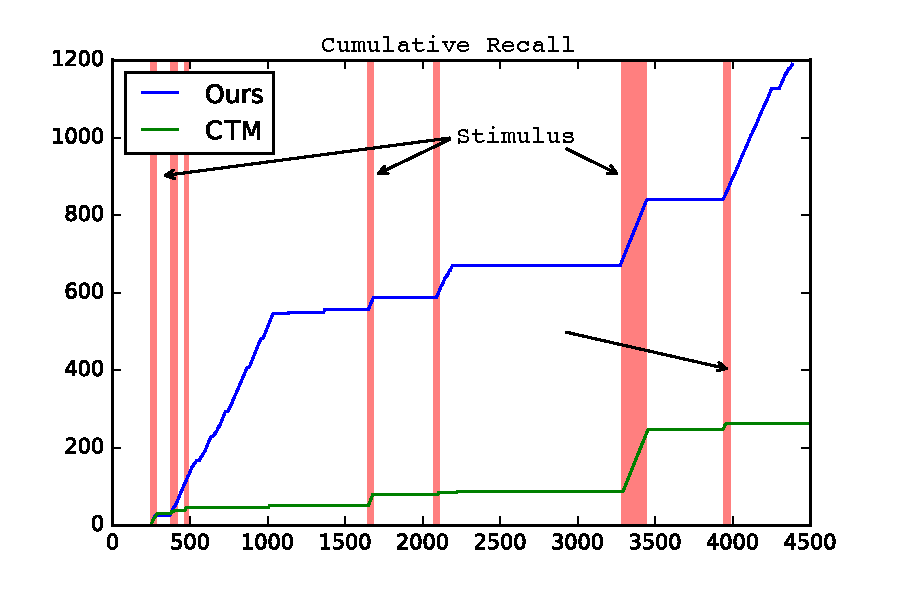
\includegraphics[width=0.8\textwidth]{loss.pdf}
\caption{不明觉厉的实验结果}
\label{result}
\end{figure}

实验结果如图\ref{result}所示。好棒棒啊,我真厉害,为自己点赞。啊,图啥意思?你问我,我问谁啊?你问我,我问谁啊?你问我,我问谁啊?你问我,我问谁啊?你问我,我问谁啊?你问我,我问谁啊?你问我,我问谁啊?你问我,我问谁啊?你问我,我问谁啊?你问我,我问谁啊?你问我,我问谁啊?你问我,我问谁啊?你问我,我问谁啊?你问我,我问谁啊?你问我,我问谁啊?你问我,我问谁啊?你问我,我问谁啊?你问我,我问谁啊?你问我,我问谁啊?你问我,我问谁啊?你问我,我问谁啊?你问我,我问谁啊?你问我,我问谁啊?你问我,我问谁啊?你问我,我问谁啊?你问我,我问谁啊?你问我,我问谁啊?你问我,我问谁啊?你问我,我问谁啊?你问我,我问谁啊?你问我,我问谁啊?你问我,我问谁啊?你问我,我问谁啊?

你问我,我问谁啊?你问我,我问谁啊?你问我,我问谁啊?你问我,我问谁啊?你问我,我问谁啊?你问我,我问谁啊?你问我,我问谁啊?你问我,我问谁啊?你问我,我问谁啊?你问我,我问谁啊?你问我,我问谁啊?你问我,我问谁啊?你问我,我问谁啊?你问我,我问谁啊?你问我,我问谁啊?你问我,我问谁啊?

你问我,我问谁啊?你问我,我问谁啊?你问我,我问谁啊?你问我,我问谁啊?你问我,我问谁啊?你问我,我问谁啊?你问我,我问谁啊?你问我,我问谁啊?你问我,我问谁啊?你问我,我问谁啊?你问我,我问谁啊?你问我,我问谁啊?你问我,我问谁啊?你问我,我问谁啊?你问我,我问谁啊?你问我,我问谁啊?你问我,我问谁啊?你问我,我问谁啊?你问我,我问谁啊?你问我,我问谁啊?你问我,我问谁啊?你问我,我问谁啊?你问我,我问谁啊?你问我,我问谁啊?你问我,我问谁啊?你问我,我问谁啊?你问我,我问谁啊?你问我,我问谁啊?你问我,我问谁啊?你问我,我问谁啊?你问我,我问谁啊?你问我,我问谁啊?你问我,我问谁啊?

不知道,真的不知道!不知道,真的不知道!不知道,真的不知道!不知道,真的不知道!不知道,真的不知道!不知道,真的不知道!不知道,真的不知道!不知道,真的不知道!不知道,真的不知道!不知道,真的不知道!不知道,真的不知道!不知道,真的不知道!不知道,真的不知道!不知道,真的不知道!不知道,真的不知道!不知道,真的不知道!不知道,真的不知道!不知道,真的不知道!不知道,真的不知道!不知道,真的不知道!不知道,真的不知道!不知道,真的不知道!不知道,真的不知道!不知道,真的不知道!不知道,真的不知道!不知道,真的不知道!不知道,真的不知道!不知道,真的不知道!

不知道,真的不知道!不知道,真的不知道!不知道,真的不知道!不知道,真的不知道!不知道,真的不知道!不知道,真的不知道!不知道,真的不知道!不知道,真的不知道!不知道,真的不知道!不知道,真的不知道!

不知道,真的不知道!不知道,真的不知道!不知道,真的不知道!不知道,真的不知道!不知道,真的不知道!不知道,真的不知道!不知道,真的不知道!不知道,真的不知道!不知道,真的不知道!不知道,真的不知道!不知道,真的不知道!不知道,真的不知道!不知道,真的不知道!不知道,真的不知道!不知道,真的不知道!不知道,真的不知道!不知道,真的不知道!不知道,真的不知道!不知道,真的不知道!不知道,真的不知道!不知道,真的不知道!不知道,真的不知道!不知道,真的不知道!不知道,真的不知道!不知道,真的不知道!不知道,真的不知道!不知道,真的不知道!不知道,真的不知道!不知道,真的不知道!不知道,真的不知道!不知道,真的不知道!不知道,真的不知道!不知道,真的不知道!不知道,真的不知道!不知道,真的不知道!不知道,真的不知道!不知道,真的不知道!不知道,真的不知道!不知道,真的不知道!不知道,真的不知道!不知道,真的不知道!不知道,真的不知道!不知道,真的不知道!不知道,真的不知道!不知道,真的不知道!不知道,真的不知道!

不知道,真的不知道!不知道,真的不知道!不知道,真的不知道!不知道,真的不知道!不知道,真的不知道!不知道,真的不知道!不知道,真的不知道!不知道,真的不知道!不知道,真的不知道!不知道,真的不知道!不知道,真的不知道!不知道,真的不知道!不知道,真的不知道!

\clearpage{\pagestyle{empty}\cleardoublepage}


%----------------------------------------------
\chapter{总结与展望}
\echapter{Summary and Prospects}
\section{本文工作总结}
\esection{Summary of the Thesis}
本文基于排队论,研究了海韵二期食堂小炒的排队策略。我们啥也没干,程序网上抄的,实验前两天跑的,论文最晚熬夜胡的。真的很无聊。真的很无聊。真的很无聊。真的很无聊。真的很无聊。真的很无聊。真的很无聊。真的很无聊。真的很无聊。真的很无聊。真的很无聊。真的很无聊。

真的很无聊。真的很无聊。真的很无聊。真的很无聊。真的很无聊。真的很无聊。真的很无聊。真的很无聊。真的很无聊。真的很无聊。真的很无聊。真的很无聊。真的很无聊。真的很无聊。

(1)科研之无聊

实验室就是大监狱,导师就是典狱长,你想出狱,典狱长就看死你。读论文,读论文,就知道读那些没用的论文。头发一天天洗漱,性功能一天天衰退,青春的滋味一点每尝到,关塔那摩的痛苦倒是分外清晰。

(2)再论科研之无聊

这些课题有意义吗?写的那些废纸有人看吗?学生几年后学到了什么呀?没!没!!没!!!除了浪费钱,浪费时间,浪费生活的美好,还有什么意义!!!

(3)终论科研之无聊

学生之科研——我要拿学位!教授之科研——我要评职称!学校之科研——自娱自乐矣!送钱到国外,版面乖乖买,仪器我也要,版面买一再赠一。

\section{研究展望}
\esection{Research Prospects}
有啥好展望的,咱都毕业了,你说你还让我展望未来研究工作,还研究你个大头鬼!大头鬼!大头鬼!大头鬼!大头鬼!大头鬼!大头鬼!大头鬼!大头鬼!大头鬼!大头鬼!大头鬼!大头鬼!大头鬼!大头鬼!大头鬼!大头鬼!大头鬼!大头鬼!大头鬼!大头鬼!大头鬼!大头鬼!大头鬼!大头鬼!大头鬼!大头鬼!大头鬼!大头鬼!大头鬼!大头鬼!大头鬼!大头鬼!大头鬼!大头鬼!大头鬼!

你敢让我再研究,我就在网上发帖!网上发帖!网上发帖!网上发帖!网上发帖!网上发帖!网上发帖!网上发帖!网上发帖!网上发帖!网上发帖!网上发帖!网上发帖!网上发帖!网上发帖!网上发帖!网上发帖!网上发帖!网上发帖!网上发帖!网上发帖!网上发帖!网上发帖!网上发帖!网上发帖!网上发帖!网上发帖!网上发帖!网上发帖!网上发帖!网上发帖!网上发帖!网上发帖!网上发帖!网上发帖!网上发帖!网上发帖!网上发帖!网上发帖!网上发帖!网上发帖!网上发帖!网上发帖!

不让我展望了是不是,好,很好,非常好!好,很好,非常好!好,很好,非常好!好,很好,非常好!好,很好,非常好!好,很好,非常好!好,很好,非常好!好,很好,非常好!好,很好,非常好!好,很好,非常好!好,很好,非常好!好,很好,非常好!好,很好,非常好!好,很好,非常好!好,很好,非常好!好,很好,非常好!好,很好,非常好!好,很好,非常好!好,很好,非常好!好,很好,非常好!好,很好,非常好!好,很好,非常好!好,很好,非常好!好,很好,非常好!好,很好,非常好!好,很好,非常好!好,很好,非常好!好,很好,非常好!好,很好,非常好!好,很好,非常好!好,很好,非常好!好,很好,非常好!好,很好,非常好!

论文终于扯完了。呵呵!呵呵!呵呵!呵呵!呵呵!呵呵!呵呵!呵呵!呵呵!呵呵!呵呵!呵呵!呵呵!呵呵!呵呵!呵呵!呵呵!呵呵!呵呵!呵呵!呵呵!呵呵!呵呵!呵呵!呵呵!呵呵!呵呵!呵呵!呵呵!

\clearpage{\pagestyle{empty}\cleardoublepage}



\bibliographystyle{plain}
\addcontentsline{toc}{chapter}{参考文献} 
\addcontentsline{toe}{chapter}{References}
\begin{thebibliography}{99}

\bibitem{momo2003} 沫沫. 革命的本钱[J]. 东方少年(快乐文学), 2003(1).

\bibitem{Khan2006} Khan K S, Wojdyla D, Say L, et al. WHO analysis of causes of maternal death: a systematic review.[J]. Lancet, 2006, 367(9516):1066-1074.

\bibitem{Marcus2015} Marcus K H. Book Review: Dance Floor Democracy: The Social Geography of Memory at the Hollywood Canteen[J]. Southern California Quarterly, 2015, 97(2):225-228.

\end{thebibliography}

\end{document}